\documentclass{fairmeta}

\usepackage{graphicx}
\usepackage{natbib}
\usepackage{appendix}
\usepackage{booktabs}
\usepackage{url}
\usepackage{xcolor}
\usepackage{tcolorbox}
\usepackage{hyperref}
\definecolor{RoyalBlue}{RGB}{65,105,225}
\definecolor{Green}{RGB}{34,139,34}
\hypersetup{
 colorlinks=true,
 citecolor=RoyalBlue,
 linkcolor=RoyalBlue,
 filecolor=magenta, 
 urlcolor=RoyalBlue
}
\usepackage{cleveref}
\usepackage{tabularx}
\usepackage{comment}
\usepackage{subfig}
\usepackage{tikz}
\usepackage{fvextra}
\newenvironment{minted}[2][]{\VerbatimEnvironment\begin{Verbatim}[fontsize=\scriptsize]}{\end{Verbatim}}
\newcommand{\setminted}[1]{}
\setminted{fontsize=\scriptsize}
\usepackage{amssymb}
\usepackage{wrapfig}

\usepackage{fontawesome}
\usepackage{pifont}

\definecolor{lvl1}{HTML}{93acf5}
\definecolor{lvl2}{HTML}{1549e4} 
\definecolor{lvl3}{HTML}{091f62} 


\newcommand{\greg}[1]{{\color{violet}\textbf{GM: #1}}}
\newcommand{\clem}[1]{{\color{orange}\textbf{CF: #1}}}
\newcommand{\tsc}[1]{{\color{blue}\textbf{托马斯·西亚罗姆:#1}}}

\newcommand{\wip}[1]{{\color{red}\textbf{#1}}}

\newcommand{\benchmark}{\textsc{GAIA}}
\newcommand{\total}{466}
\newcommand{\test}{300}
\newcommand{\dev}{166}
\newcommand{\humanscore}{92\%}

\title{\begin{center}
 \benchmark{}: \\ 通用 \textbf{AI} 助手基准\end{center}
}

\author[1]{Gr\'egoire Mialon}
\author[2]{Cl\'ementine Fourrier}
\author[3]{Craig Swift}
\author[2]{Thomas Wolf}
\author[1]{Yann LeCun}
\author[4]{Thomas Scialom}

\affiliation[1]{FAIR, Meta}
\affiliation[2]{HuggingFace}
\affiliation[3]{AutoGPT}
\affiliation[4]{GenAI, Meta}

\abstract{

本文介绍 \benchmark{}，一个面向通用 AI 助手的基准。若系统能够稳定解决其中的问题，说明其通用助手能力已经取得实质进展。\benchmark{} 包含现实世界问题，需要推理、多模态处理、网页浏览以及熟练使用通用工具等基本能力。
\benchmark{} 的问题对人类而言在概念上并不复杂，但对当前多数先进 AI 系统仍然很有挑战性：人类受试者得分为 92\%，而配备插件的 GPT-4 得分为 15\%。
这一明显差距与近期大型语言模型在法律、化学等需要专门技能的任务上超过人类的趋势形成对比。
\benchmark{} 的设计理念也不同于许多现有 AI 基准：它并不追求对人类更难的任务，而是关注普通人可以完成、但 AI 助手仍难以可靠完成的问题。
我们认为，通用人工智能的出现取决于系统能否在这类问题上表现出接近普通人的稳健性。为构建 \benchmark{}，我们设计了 466 个问答样本。我们公开全部问题，并保留其中 300 个问题的答案用于排行榜评测；数据集可通过 \href{https://huggingface.co/gaia-benchmark}{Hugging Face 项目页}获取。

}

\date{\today}
\correspondence{\email{\{gmialon,tscialom\}@meta.com}, \email{clementine@huggingface.co}}

\metadata[Code]{\url{https://huggingface.co/gaia-benchmark}}



% Chinese translation support
\usepackage{xeCJK}
\setCJKmainfont{FandolSong-Regular.otf}[ItalicFont=FandolKai-Regular.otf]
\setCJKsansfont{FandolHei-Regular.otf}
\setCJKmonofont{FandolFang-Regular.otf}
\XeTeXlinebreaklocale "zh"
\XeTeXlinebreakskip = 0pt plus 1pt
\renewcommand{\abstractname}{摘要}
\renewcommand{\figurename}{图}
\renewcommand{\tablename}{表}
\renewcommand{\refname}{参考文献}
\renewcommand{\contentsname}{目录}
\makeatletter
\AtBeginDocument{%
 \@ifundefined{crefname}{}{%
 \crefname{figure}{图}{图}%
 \Crefname{figure}{图}{图}%
 \crefname{table}{表}{表}%
 \Crefname{table}{表}{表}%
 \crefname{section}{节}{节}%
 \Crefname{section}{节}{节}%
 \crefname{appendix}{附录}{附录}%
 \Crefname{appendix}{附录}{附录}%
 \crefname{algocf}{算法}{算法}%
 \Crefname{algocf}{算法}{算法}%
 }%
 \@ifundefined{SetAlgorithmName}{}{\SetAlgorithmName{算法}{算法}{算法列表}}%
}
\makeatother
\raggedbottom

\begin{document}


\maketitle


\section{导言}


\begin{figure}[h!]
 \centering
 \begin{tcolorbox}[colframe=RoyalBlue, colback=white]
 \begin{center}
 \textbf{\textcolor{lvl1}{Level 1}} 
 \end{center}
 \textbf{问题:}
 根据 NIH 网站，从 2018 年 1 月到 5 月，H. pylori 在寻常痤疮患者中的临床试验实际招募人数是多少?
 \\
 \textbf{标准答案:} 90
 \begin{center}
 \textbf{\textcolor{lvl2}{Level 2}} 
 \end{center}
 \begin{minipage}[c]{0.2\textwidth}
 \centering
 \begin{tikzpicture}
 \draw[rounded corners=5pt,line width=2pt, color=lvl2] (0,0) rectangle (2.3cm, 3.0cm);
 \clip[rounded corners=5pt] (0,0) rectangle (2.3cm, 3.0cm);
 \node at (1.15cm, 1.5cm) {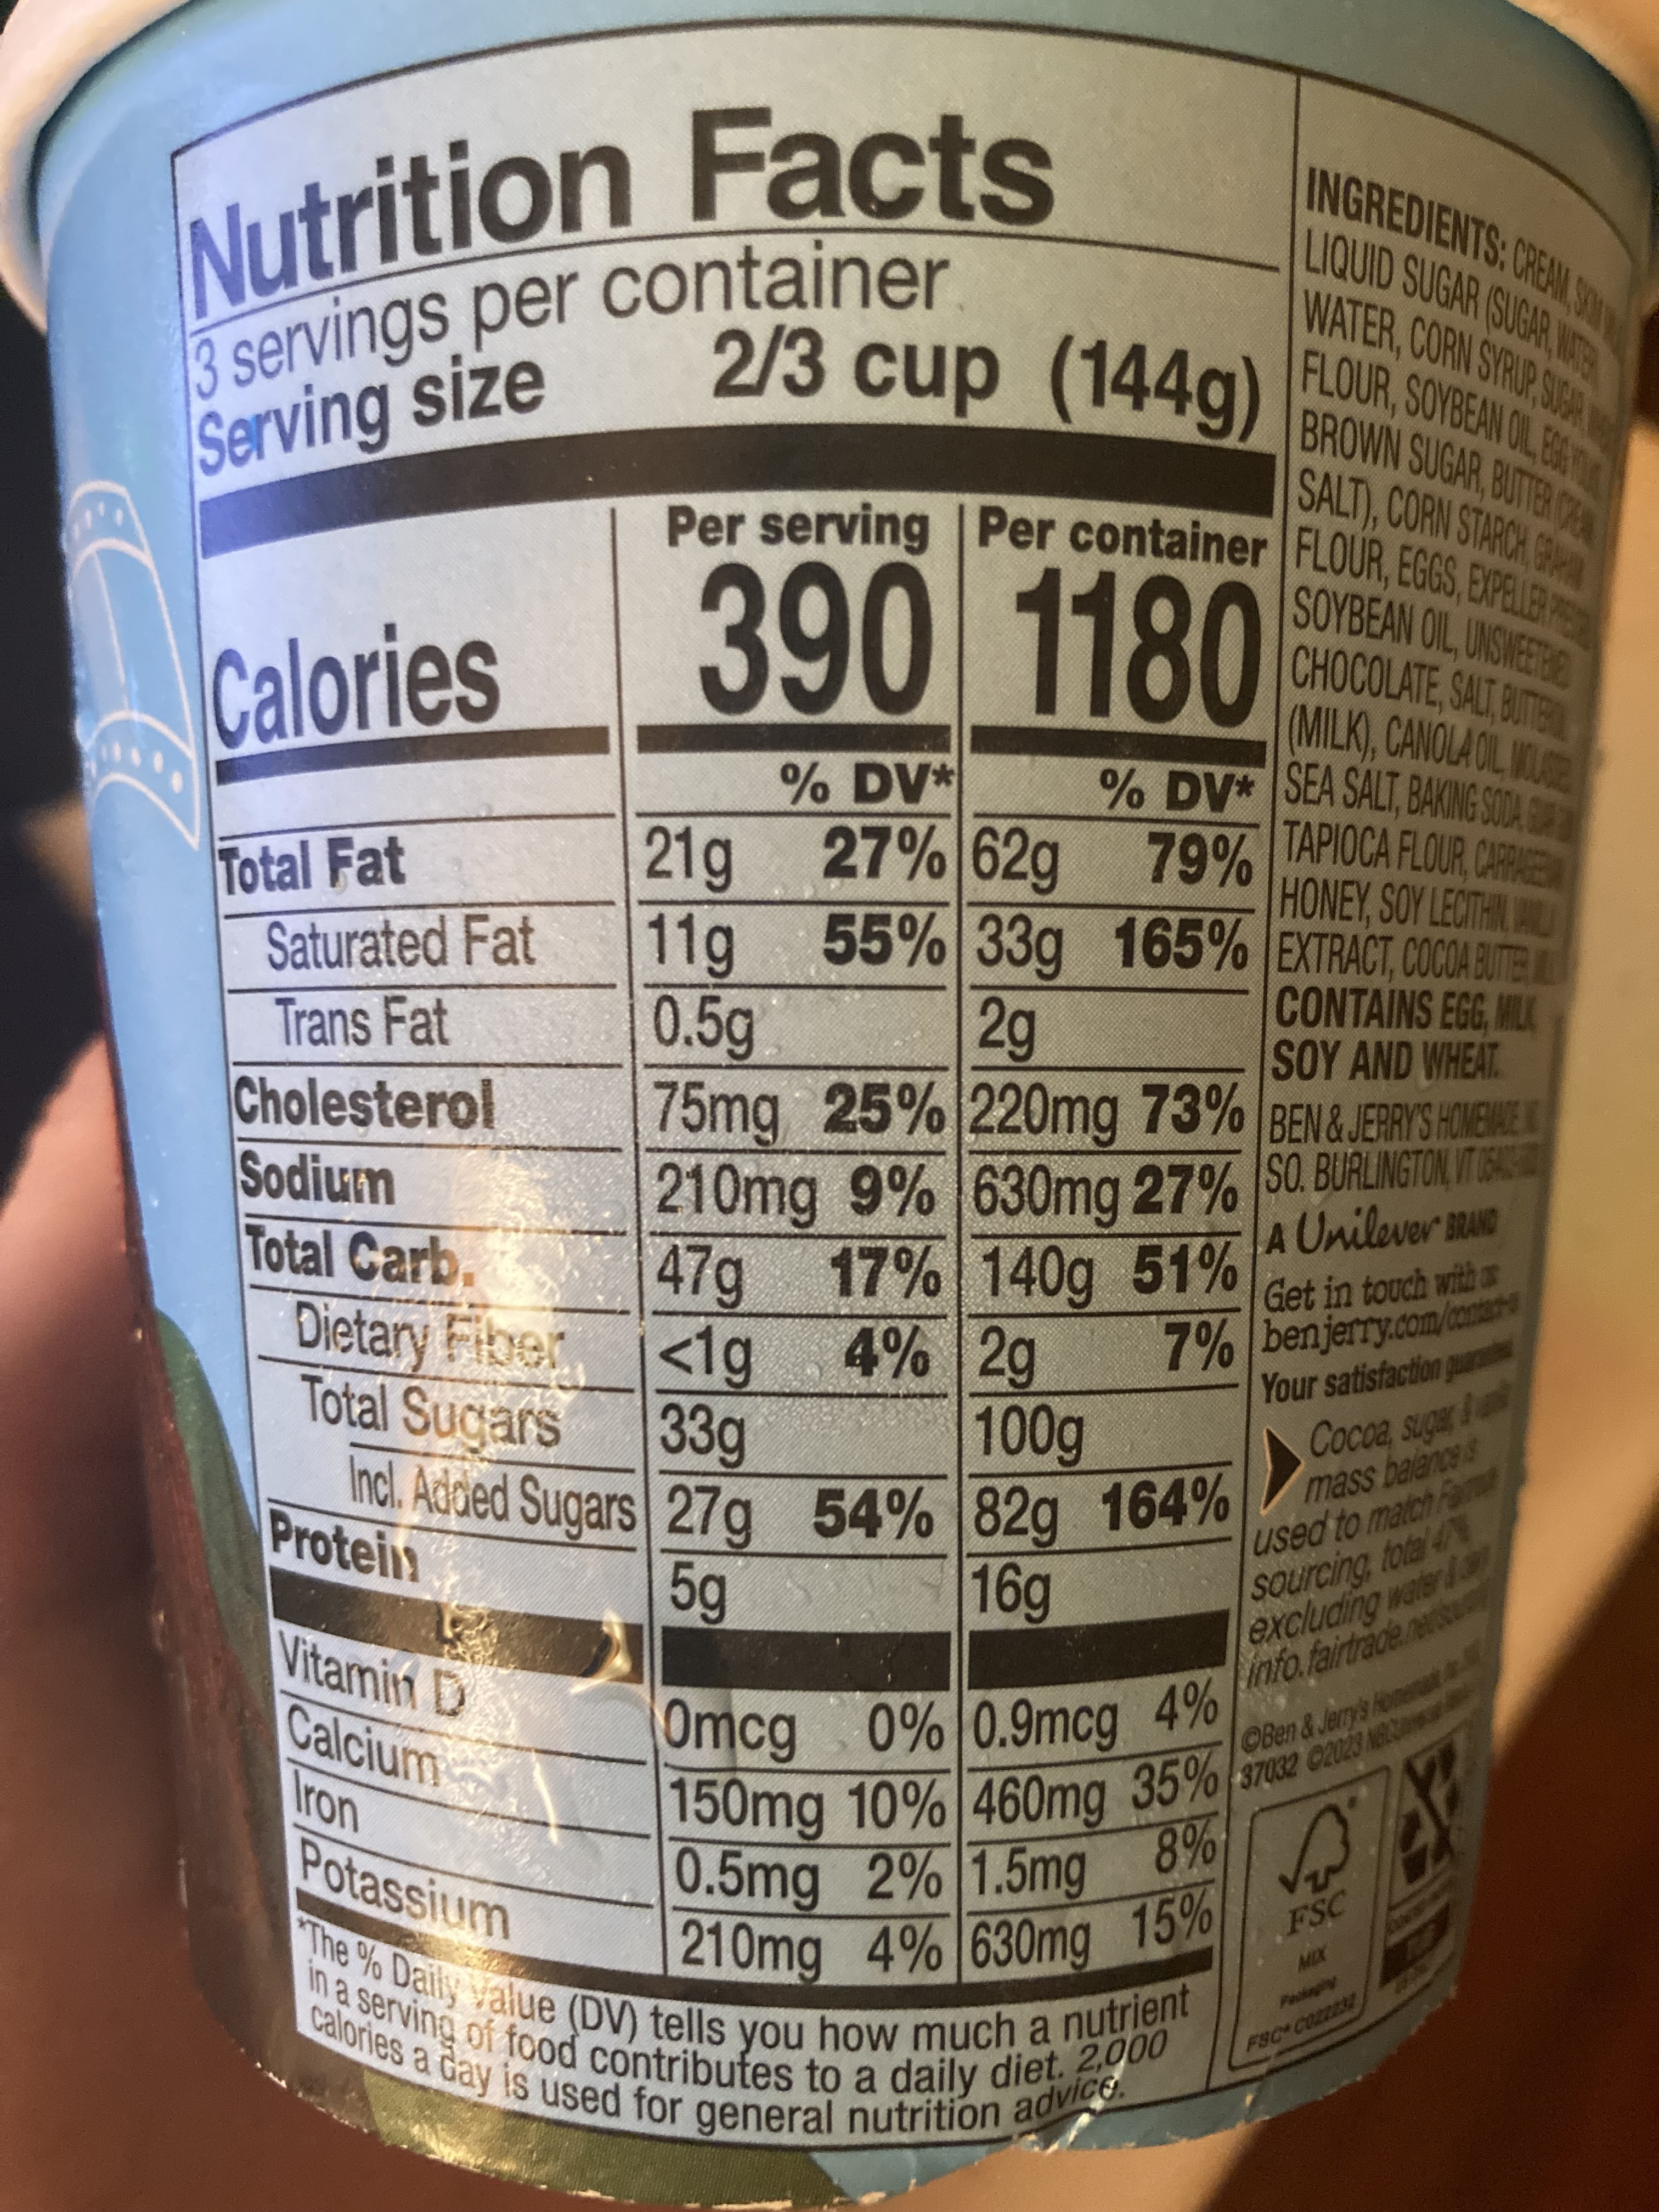
\includegraphics[width=2.3cm,height=3.0cm]{figures/ice_cream.jpg}};
 \end{tikzpicture}
 \end{minipage}
 % \hfill
 \begin{minipage}[c]{0.79\textwidth}
 \textbf{问题:} 如果这一品脱食品全部按冰淇淋计算，并按 2020 年维基百科记录的美国联邦标准判断，它的乳脂含量比标准高出或低于多少个百分点? 答案写作带正负号的数字，并四舍五入到小数点后一位。
 \\
 \textbf{标准答案:} +4.6 
 \end{minipage}
 \begin{center}
 \textbf{\textcolor{lvl3}{Level 3}} 
 \end{center}
 \textbf{问题:}
 在 NASA 2006 年 1 月 21 日的“每日天文图片”中可以看到两名宇航员，其中一名看起来明显小于另一名。截至 2023 年 8 月，在这名较小宇航员所属的 NASA 宇航员组中，哪位宇航员在太空停留的时间最短? 他在太空停留了多少分钟，四舍五入到最接近的整数分钟? 不包括从未进入太空的宇航员。请给出宇航员姓氏，并用分号与分钟数分隔；分钟数使用千位分隔符。
 \\
 \textbf{标准答案:} White; 5,876
 \end{tcolorbox}
 \caption{\benchmark{} 的样例问题。完成这些任务需要推理、多模态处理和熟练使用工具等基础能力。答案是明确的，并且在设计上不太可能以纯文本形式出现在训练数据中。部分问题还附带图像等额外证据，以贴近真实使用场景，并便于更好地控制问题内容。}
 \label{fig:demo_questions}
\end{figure}

大型语言模型（LLM）为通用系统打开了新的可能。近期模型~\citep{openai2023gpt4, anthropic2023claude2, anil2023palm, touvron2023llama2} 已经具备流畅的语言能力、丰富的知识，并在一定程度上与人类偏好对齐~\citep{ouyang2022training}；它们还可以在零样本或少样本设置下接入网页浏览器、代码解释器等工具~\citep{mialon2023augmented,brown2020language}。然而，如何评价这类系统仍是开放问题：随着新能力不断涌现，LLM 正以越来越快的速度突破既有 AI 基准~\citep{_kiela-etal-2023-plottingprogress}。

 
为了构造更有挑战性的基准，一个自然趋势是寻找对人类也越来越困难的任务，例如更复杂的 STEM 或法律考试，或者更复杂的生成任务，如写出一本连贯的书。但对人类困难，并不意味着对近期系统也困难。例如 MMLU 和 GSM8k~\citep{_hendrycks-etal-2021-measuring-mmlu, cobbe2021training} 原本具有挑战性，如今已经接近被解决。\footnote{GPT4 在 MMLU 上达到 86.4\%。相比之下，非专家人类在该基准上的准确率仅为 34.5\%，专家级人类表现估计为 89.8\%。} 这既与 LLM 能力快速提升有关，也可能受到数据污染影响。\footnote{\href{https://www.surgehq.ai/blog/hellaswag-or-hellabad-36-of-this-popular-llm-benchmark-contains-errors}{See for example the case of Hellaswag.}}
开放式生成通常需要人工评价或基于模型的评价~\citep{zheng2023judging}。随着任务复杂度提高，人工评价会越来越难以扩展，例如当输出很长或需要特殊技能时：我们该如何评价 AI 生成的一本书，或评价只有极少数人能解出的数学题解? 另一方面，基于模型的评价天然依赖更强的模型，因此难以评价新的最先进模型，还可能引入不易察觉的偏差，例如偏好排在第一位的候选答案~\citep{zheng2023judging}。
总体来看，评价新的 AI 系统需要重新思考基准设计~\citep{chollet2019measure}。

另一条思路是保留较低的人类难度，同时要求 AI 系统精确执行复杂动作序列；这类任务通常具有较大的组合空间。任务产出只有在步骤全部成功后才能得到，而且容易验证，这类似于工作量证明算法~\citep{jakobsson1999proofs,dwork1993pricing}：计算机需要求解一个复杂问题，但解本身易于核验。AI 助手任务天然符合这一标准，因为它们需要进入多样且不确定的现实世界，同时又扎根于实际使用场景。

沿着这一方向，我们提出 \benchmark{}，一个面向通用 AI 助手的基准，包含 \total{} 个人工设计的问题及其答案，并给出相应的设计方法。这些问题构造成本相对可控，却能给 AI 系统带来挑战；对 LLM 来说，其中大多数需要复杂的生成过程，但最终都对应唯一的事实性答案，因此可以进行简单而稳健的自动评价。

\benchmark{} 试图通过以下设计避开当前 LLM 评价中的常见陷阱：
\begin{itemize}
 \item[-] 现实世界中的挑战性问题。例如，LLM 通常需要浏览开放且不断变化的网络、处理多模态信息，或经过多个推理步骤才能回答问题。相比之下，许多 LLM 基准非常具体，或被限制在封闭的合成环境中。
 
 \item[-] 易解释性。任务在概念上简单，非专家标注者几乎可以取得满分；同时，任务数量较少但经过精细筛选，并可配合推理轨迹进行分析。这不同于一些汇总式基准，后者可能缺乏效率和可靠性~\citep{perlitz2023efficient}。

 \item[-] 难以投机取巧。回答问题需要成功完成若干步骤，而这些步骤差异很大，难以通过暴力枚举解决。推理轨迹可检查、答案要求精确，并且答案通常不会以纯文本形式出现在互联网上，这些因素都有助于降低数据污染风险。相比之下，多项选择题（\textit{e.g.}, MMLU）更难判断污染，因为错误的推理过程也可能碰巧得到正确选项。
 
\item[-] 使用简单。关键在于，我们问题的答案都是事实性、简短且无歧义的，因此可以进行简单、快速、可核验的评价。问题设计为零样本回答，以减少评价设置带来的影响。许多 LLM 基准则对实验设置较敏感，例如提示数量、提示形式
~\citep{liang2022holistic}（第 8.2 节）或具体的基准实现。\footnote{\url{https://huggingface.co/blog/evaluating-mmlu-leaderboard}}
\end{itemize}

尽管最强的 LLM 已经能解决许多人类觉得困难的任务，它们在 \benchmark{} 上仍表现不佳。即便接入工具，GPT4 在最简单任务上的成功率也不超过 30\%，在最难任务上为 0\%。
与此同时，人类答题者的平均成功率为 \humanscore{}。因此，一个能够解决 \benchmark{} 的系统可以放在 t-AGI 的语境下评价：\footnote{根据\url{https://www.alignmentforum.org/posts/BoA3agdkAzL6HQtQP/clarifying-and-predicting-agi}中的定义，t-AGI 指在多数任务上能够击败多数给定时间 $t$ 完成任务的人类专家的系统。} 人类回答最简单问题通常需要 6 分钟，回答最复杂问题需要 17 分钟。从另一个相关视角看，这样的系统在 \citet{morris2023levels} 近期提出的框架中也可被视为有能力的通用 AI；而 ChatGPT~\citep{openai2023gpt4} 仍低一个等级，这也说明 \benchmark{} 捕捉到了当前 AI 研究尚未解决的一类能力缺口。
本文介绍 \benchmark{} 的构成和设计选择，并说明如何设计问题及其相关挑战，使社区能够继续扩展该基准，覆盖工具使用安全、多模态能力等新兴问题。
我们还分析了迄今若干强助手系统的成功与不足，讨论为 LLM 接入工具后的能力边界。
我们发布 \dev{} 个带答案的问题作为开发集，
并保留其余 \test{} 个无答案问题用于排行榜评测。
我们希望这一基准能为 NLP 及更广泛领域中的开放式生成评价提供一个可操作的方向；能够解决 \benchmark{} 的系统，也将代表下一代 AI 系统的一项重要进展。

\section{相关工作}
\paragraph{评价大语言模型.} 随着 LLM 能力快速提升，基准正以越来越快的速度饱和。例如，阅读理解在几年前仍是一项有挑战性的任务~\citep{rajpurkar2016squad}。\citet{_wang-etal-2018-glue} 提出的通用语言理解评价基准（GLUE）在发布一年内就被模型超过人类水平；其后继版本 SuperGLUE~\citep{_wang-etal-2019-superglue} 也只坚持了两年多。更一般地说，静态基准被饱和并达到人类水平所需的时间逐年缩短，这一点在 \citet{_kiela-etal-2023-plottingprogress} 中也有清楚体现。
在寻找更难评价任务时，一个自然方向是考察法律、科学等领域的专业知识。MMLU~\citep{_hendrycks-etal-2021-measuring-mmlu} 就是一个例子，它包含 15,000 多个问题，覆盖 STEM、人文、社会科学等 57 个学科。
然而，LLM 已经在这些任务上超过人类表现，
甚至有报道称它们已经达到可以较可信地通过美国律师考试~\citep{openai2023gpt4} 或超过 USMLE 及格线的阶段；USMLE 是美国用于评估临床能力并授予执业资格的考试项目~\citep{nori2023capabilities}。
更全面地评价 LLM 及其更广泛的对话能力，已有方向包括：（i）整合多种评价集~\citep{_gao-etal-2021-harness,_liang-etal-2022-holistic,_srivastava-etal-2023-bigbench}，但这类评价往往难以有意义地汇总，也容易受到数据泄漏污染；（ii）人工评价，但其耗时且难以扩展；（iii）使用基于模型的评价来缓解扩展性问题~\citep{zheng2023judging}。不过，后一种方案依赖比被评模型更强的 LLM（通常是 GPT4），评价质量也会受到评价者 LLM 自身缺陷影响，而这些缺陷并不总是显而易见，可能导致细微但错误的结果。


\paragraph{评价通用助手。}
虽然已有大量工作试图将大语言模型转化为通用助手（见附录~\ref{sec:extended_related_work} 的讨论），相应评价仍然滞后。
大多数评价依赖封闭系统、特定 API 调用以及达到答案的某种“正确方式”，或者只是重新利用已有评价数据集。例如，ToolQA~\citep{_zhuang-etal-2023-toolqa} 和 Gentopia~\citep{_xu-etal-2023-gentopia} 将现有数据集与人工标注结合起来（如 MMLU、MATH 等），这既可能在训练期间受到污染，也不能确保工具使用本身确实被测试到。Gorilla~\citep{_patil-etal-2023-gorilla} 引入 APIBench，用于测试类智能体系统调用其特定 API 的能力；API-Bank~\citep{_li-etal-2023-apibank} 也类似，提供一个 API 池帮助 LLM 完成评价。AgentBench~\citep{liu2023agentbench} 更通用一些，提供若干封闭环境，让助手型 LLM 在其中回答用户查询（从 Unix shell 到 WebShopping API）。然而，这类评价依赖封闭环境，因此可能评估的是助手是否学会了使用特定 API，而不是在现实世界交互中的更一般能力。
相反，\benchmark{} 不预先规定可用 API，而是依赖与现实世界的交互。
OpenAGI~\citep{_ge_2023_openagi} 同时提出平台和基准，由跨模态、跨能力的多步骤任务组成，与我们的工作更接近。\benchmark{} 与其核心区别在于，OpenAGI 的任务更关注当前模型能力，而 \benchmark{} 面向即将出现的能力进展。

\section{\benchmark{}}

本节介绍 \benchmark{} 的设计和内容，以及创建问题时使用的准则和相关挑战。

\subsection{一个便于使用且具有挑战性的通用 AI 助手基准}

\paragraph{\benchmark{} 是什么，如何使用?} \benchmark{} 是一个面向通用助手问题的 AI 系统基准。它包含 \total{} 个由人类设计并标注的问题。这些问题以文本为主，有时附带文件（例如图像或电子表格），覆盖日常个人任务、科学和一般知识等多种助手使用场景。问题被设计为只接受一个简短且正确的答案，因此易于核验。使用 \benchmark{} 时，只需将问题及其附带证据以零样本方式提示给 AI 助手。
要在 \benchmark{} 上取得满分，需要多种基础能力（见\Cref{sec:composition}）。我们在补充材料中提供问题及其元数据。


\begin{figure}[h!]
 \centering
 \begin{tcolorbox}[colframe=RoyalBlue, colback=white]
 \textbf{系统提示:} 你是一个通用 AI 助手。我会问你一个问题。请报告你的思路，并用以下模板结束回答：FINAL ANSWER: [YOUR FINAL ANSWER].\\
 最终答案应当是一个数字、尽可能少的词，或由数字和/或字符串组成的逗号分隔列表。\\
 如果要求数字，除非另有说明，不要在数字中使用逗号，也不要使用 \$ 或百分号等单位。\\
 如果要求字符串，除非另有说明，不要使用冠词，也不要使用缩写（例如城市缩写）；数字请用纯文本写出。\\
 如果要求逗号分隔列表，请根据列表元素是数字还是字符串应用上述规则。
 \\
 \\
 \begin{minipage}{0.75\textwidth}
 \textbf{\benchmark{} 问题:} 所附的 Excel 文件包含一家本地快餐连锁店各菜单项的销售情况。该连锁店食品项（不包括饮料）的销售总额是多少? 答案保留两位小数。
 \end{minipage}
 \hfill
 \begin{minipage}{0.2\textwidth}
 \centering
 
\includegraphics[scale=.08]{figures/xlsx_icon.png}
 \small{\texttt{uploaded.xlsx}}
 \end{minipage}
 \\
 \\
 \textbf{GPT4（高级数据分析模式）:} 
 \\
 \\ 执行代码:
 \begin{tcolorbox}[colframe=RoyalBlue, colback=gray!10]
 \begin{minted}{python}
import pandas as pd

# Load the Excel file
file_path = '/mnt/data/uploaded.xlsx'
df = pd.read_excel(file_path)
\end{minted}
\end{tcolorbox}
执行代码:
\begin{tcolorbox}[colframe=RoyalBlue, colback=gray!10]
\begin{minted}{python}
# Calculate the total sales from food items (not including drinks i.e., Soda)
total_food_sales = df[
 ['Burgers', 'Hot Dogs', 'Salads', 'Fries', 'Ice Cream']
].sum().sum()

# Format the result to USD, with a dollar sign and two decimal places
total_food_sales_formatted = f"${total_food_sales:,.2f}"
\end{minted}
\end{tcolorbox}
最终回答:\texttt{\$89706.00} \hspace{1cm}\textbf{标准答案:} \texttt{89706.00} \textcolor{Green}{{\Large \checkmark}}


 \end{tcolorbox}
 \caption{回答 \benchmark{} 问题时，GPT4（本例中配备代码解释器）等 AI 助手需要完成多个步骤，并可能需要使用工具或读取文件。}
 \label{fig:demo_gpt4}
\end{figure}



\paragraph{设计选择.} \benchmark{} 的设计来自对现有 AI 基准不足的反思，尤其是对 LLM 评价缺陷的分析。

第一项原则是选择概念上简单、对人类可能繁琐但形式多样的问题。这些问题扎根于现实世界，并且对当前 AI 系统仍有挑战。它们主要考察推理、多模态理解以及潜在的多工具使用等基础能力，而不是专业技能，从而更接近快速适应能力~\citep{chollet2019measure}。问题通常要求从不同来源查找、转换并整合信息，例如用户提供的文件，或开放且不断变化的网络，最终得到精确答案。
以上方第一个样例问题（\Cref{fig:demo_questions} 中 Level 1）为例，LLM 通常需要浏览网页、找到对应研究，再定位正确的招募人数。这与“不断寻找对人类更难的任务”的基准趋势相反，也不同于只在纯文本或人工环境中运行的评价。

我们的第二项原则是可解释性。
\benchmark{} 的问题数量有限，相比大型汇总式基准更便于使用~\citep{perlitz2023efficient}。任务在概念上较简单（人类成功率为 \humanscore{}），因此用户也更容易理解模型的推理轨迹。
以\Cref{fig:demo_questions}中的 Level 1 问题为例，推理轨迹主要包括访问正确网站并报告正确招募人数，核验起来很直接。

第三项原则是尽量避免记忆。\benchmark{} 要求系统规划并成功完成若干步骤，因为按设计，最终答案不会直接出现在当前预训练数据中。准确率提升应反映系统真实能力的提升。由于任务类型多样且动作空间很大，除非作弊，否则难以通过暴力方式完成，例如直接记住标准答案。数据污染仍可能导致意外记忆，但答案所要求的精确性、推理轨迹可检查，以及答案不以纯文本形式出现在互联网上，都有助于缓解这一问题。
相比之下，多项选择题会让污染评估更困难，因为错误的推理轨迹仍可能选中正确选项。
如果即便有这些缓解措施仍发生严重记忆，也可以依据我们在\Cref{sec:guidelines}中提供的准则较容易地构造新问题。

最后一项原则是易用性。我们的任务只是一个简单提示，有时附带文件。关键在于，答案是事实性、简短且无歧义的，因此可以进行简单、快速、可核验的评价。问题设计为零样本回答，以降低评价设置的影响。相反，许多 LLM 基准对实验设置较敏感，例如提示数量和提示形式~\citep{liang2022holistic}（第 8.2 节），或具体基准实现。


\subsection{评价} \benchmark{} 支持自动、快速和事实性的评价。除非另有说明，每个问题都要求给出一个答案：字符串（一个或少数几个词）、数字，或由字符串和浮点数组成的逗号分隔列表。每个问题只有一个正确答案。因此，评估通过模型答案与标准答案之间的近似精确匹配完成，并根据答案类型进行必要的归一化，见\Cref{fig:demo_gpt4}。实践中，GPT4 级别的模型很容易遵循这一格式。我们同时提供评分函数和\href{https://huggingface.co/gaia-benchmark}{排行榜}。

\subsection{\benchmark{} 的组成}
\label{sec:composition}

本小节介绍我们为 \benchmark{} 设计的 \total{} 个问题。

\vspace{-0.2cm}

\paragraph{能力覆盖。} 在 \benchmark{} 上取得满分需要较强的推理、多模态理解、编码能力和通用工具使用能力，\textit{e.g.} 网页浏览；更精确的定义见\Cref{sec:extended_description}。我们还包含需要处理多种数据模态的问题，例如 PDF、电子表格、图像、视频或音频，其分布见\Cref{sec:extended_description}（\Cref{fig:file_types}）。\Cref{fig:gaia_overview}（左）概述了这些能力。虽然网页浏览是 \benchmark{} 的关键组成部分，但我们不要求助手执行“点击”以外的动作，例如上传文件、发表评论或预订会议。如何在真实环境中测试这些能力，同时避免网站本身变化带来的干扰，需要更谨慎的设计，我们将其留给未来工作；读者也可参考近期为 LLM 智能体提出的封闭环境~\citep{liu2023agentbench}。我们没有更细地划分解题所需能力，因为大多数问题都可以通过不同能力组合解决。例如，某个证据可能被 LLM 助手正确记住，也可能通过网络搜索检索得到。
特别地，我们没有对 LLM 工具使用进行精细度量；相关工作可参考~\citet{xu2023tool,li2023apibank}。

\begin{figure}
 \centering
 \begin{minipage}[c]{0.475\textwidth}
 \includegraphics[width=\textwidth,keepaspectratio]{figures/capabilities_histogram.pdf}
 \end{minipage}
 \begin{minipage}[c]{0.48\textwidth}
 \includegraphics[width=\textwidth,keepaspectratio]{figures/gaia_overview.pdf}
 \end{minipage}
 \caption{左：至少需要某项能力的问题数量。右：每个点对应一个 \benchmark{} 问题；在同一位置，点的大小与问题数量成正比，为保证可读性，仅显示问题数量最多的级别。这两张图都基于人类标注者回答问题时报告的信息；AI 系统可能采用不同路径。}
 \label{fig:gaia_overview}
\end{figure}

\vspace{-0.2cm}

\paragraph{递增难度。} 根据解题所需步骤数量以及所需不同工具数量，问题可分为三个难度递增的级别。步骤或工具当然没有唯一的定义，同一个问题也可能有多种解法。因此，我们依据标注者在设计问题时使用的步骤数和工具数进行分级。\Cref{fig:gaia_overview} 中的工具总是关联到一种或多种能力（见\Cref{sec:extended_description}）。我们大致使用以下定义为问题分配级别：
\begin{itemize}
 \item[-] \textbf{Level 1} 问题通常不需要工具，或最多需要一个工具，步骤数不超过 5 个。
 \item[-] \textbf{Level 2} 问题通常需要更多步骤，大约 5 到 10 步，并需要结合不同工具。
 \item[-] \textbf{Level 3} 问题面向接近完美的通用助手，可能需要较长行动序列、任意数量的工具，以及对开放世界的访问。
\end{itemize}

这些级别的示例见\Cref{fig:demo_questions}。这些定义不是硬性规则：例如，一个少于 $10$ 个标注步骤但需要复杂网页导航的问题，可能被归为 Level 3 而不是 Level 2。我们在第~\ref{sec:evaluation} 节中验证这一难度定义。

\paragraph{所需能力分布。} 虽然 \benchmark{} 以现实世界中的助手问题为目标，我们也包含一些可能让身体障碍者受益的任务，例如在短音频文件中查找某条信息。最后，我们尽力覆盖多种主题领域和文化，但数据集语言仍仅限英语（见\Cref{sec:limitations}）。

\subsection{构建和扩展 \benchmark{}}
\label{sec:guidelines}

本小节介绍问题设计和标注流程，并特别讨论其中的挑战。我们希望这些经验有助于社区继续建设 \benchmark{}。


\paragraph{设计问题.}

我们的问题都由人类创建。\footnote{更准确地说，它们来自作者团队协作，以及 Surge AI 对标注者的付费支持。} 作者首先设计初始问题，并将这些问题和说明作为示例提供给标注者（见\Cref{sec:extended_protocol}），以生成更多问题。
问题基于一个或多个事实来源，并常在题干中明确说明，以避免歧义。可靠事实来源通常是不太可能很快消失的网页，\textit{e.g.} 维基百科、Papers With Code 或 arXiv。在其他情况下，事实来源会作为问题附件直接提供，\textit{e.g.} 一个 PDF 文档或一个小谜题。我们没有规定固定的事实来源清单，以保持问题多样性并减少记忆风险。除谜题外，多数问题都要求查找并可能整合来自不同事实来源的信息，从而得出具体答案。换言之，问题创建者会提供答案元数据，包括需要哪些工具、采取了哪些步骤，以及回答所需时间，见\Cref{tab:annotated_question}（\Cref{sec:extended_description}）。

\paragraph{验证问题.} 拟订问题的大部分工作在于确保问题无歧义，\textit{i.e.} 能够被快速地进行事实性评价，因此必须保持这一性质。歧义可能非常微妙，对问题创建者来说并不总是明显。
例如，如果一个问题没有为网页指定一个版本，而回答问题所需的信息在其他版本中则不同，那么这个问题就模糊不清了。
因此，我们要求两位新的标注者独立回答每个问题；如果最初标注者和两位新标注者得到相同答案，该问题就通过验证。若标注者意见不一致，问题通常只需简单修正；否则会被删除。因此，在保持问题趣味性和多样性的同时自动生成问题并不容易。验证阶段统计见\Cref{tab:ambiguity_stats}（\Cref{sec:extended_description}）：其余问题中有 68\% 需要修正或删除。
尽管问题在概念上简单，标注者仍可能犯意想不到的错误。我们估计标注者成功率为 \humanscore{}，并将其作为 \benchmark{} 的人类基线；该数值接近满分，表明 \benchmark{} 对非专家来说较简单。我们估计，提出一个问题并由两名补充标注者验证和可能修订，约需要两小时标注者时间。



\paragraph{依赖网络带来的挑战。} 当事实来源托管在网络上时，问题设计会变得更微妙。
首先，证据可能随时间变化。例如，维基百科条目可能在问题创建与 AI 助手被提问之间发生更新，并删除回答所需证据。对于这类问题，通常必须明确指定证据版本，例如页码。
实践中，我们发现该基准对这类变化较稳健，因为我们尽量依赖能经受时间考验的证据。
其次，一些网站所有者希望通过 \texttt{robots.txt} 防止 bots 访问其网站的部分或全部内容。虽然这更像是一种限制而非硬性要求，但显然应该遵守。例如，OpenAI 向希望禁止 GPT4 访问其网站的所有者提供了如何修改 \texttt{robots.txt} 的说明。因此，我们会检查证据所在网站的相关部分是否不受限制。

\section{\benchmark{} 上的 LLM 结果}
\label{sec:evaluation}

\vspace{-.2cm}
在 \benchmark{} 上评价 LLM 只需要能够调用模型，\textit{i.e.} 具备 API 访问能力。我们在提问前使用统一的前缀提示，并在其中规定输出格式，以便提取最终答案，见~\Cref{fig:demo_gpt4}。我们评价了 GPT4~\citep{openai2023gpt4} 在有插件和无插件两种设置下的表现，\footnote{\url{https://openai.com/blog/chatgpt-plugins}} 也评价了以 GPT4 为后端的 AutoGPT。\footnote{\url{https://github.com/Significant-Gravitas/Auto-GPT}，所评估 AutoGPT 版本的提交哈希为：\texttt{ed172dec1947466cc0942abf75bb77b027cd433d}.} 目前 GPT4 插件需要人工选择（见下文），而 AutoGPT 可以自动完成选择。我们的非 LLM 基线包括人工标注者和网络搜索。对于网络搜索基线，我们将问题输入搜索引擎，并检查是否能从第一页结果中推断出答案；这有助于判断问题答案是否能直接在网上找到。只要模型提供 API，我们就运行三次并报告平均结果。

\vspace{-.2cm}

\paragraph{GPT4 插件。} 目前还没有可通过 API 调用插件的 GPT4，因此我们使用人工方式在 ChatGPT 中查询。写作时，用户需要手动选择“高级数据分析”模式（具备代码执行和文件读取能力）以及最多三个第三方插件。我们要么使用高级数据分析模式，要么根据任务最关键的能力选择第三方插件；常用插件包括链接读取、网页浏览和计算工具。遗憾的是，插件会频繁在商店中变化或消失，因而很难长期使用一组稳定插件。GPT4 官方搜索工具也曾被移除，因为它可能绕过付费墙，直到近期才被重新引入。因此，带插件 GPT4 的分数更像是对 GPT4 潜力的“oracle”估计：假设插件稳定且能自动选择，而不是一个易复现结果。

\vspace{-.2cm}

\begin{figure}[h!]
 \centering
 \includegraphics[scale=.4]{figures/gaia_results_with_times.pdf}
 \caption{每种方法在各级别上的分数和答题时间。如正文所述，GPT4+插件的分数应视为一个 oracle 估计，因为插件是按问题人工选择的。人类得分是我们的标注者在验证问题时取得的分数。}
 \label{fig:eval_results}
\end{figure}

\vspace{-0.4cm}

\paragraph{结果。} 评价结果见\Cref{fig:eval_results}，更详细的信息在\Cref{tab:detailed_eval_results}（\Cref{sec:extended_evaluation}）中给出。我们提出的难度分级与当前模型性能相关；无论从所需步骤数还是所需能力种类看，这都支持了分级设计的有效性。人类在所有级别上表现都很好，但当前最强的 LLM 仍表现有限。总体而言，\benchmark{} 能够区分不同能力水平的助手，同时也为未来数月甚至数年的改进留下了足够空间。

\begin{wrapfigure}{r}{0.56\textwidth}
 \centering
 \includegraphics[scale=.33]{figures/gaia_results_per_capability_v2.pdf}
 \caption{不同 LLM 在 Level 1 各能力类别上的得分。非工具模型在“多种文件类型读取”和“多模态”上的非零分数，来自一些可用不同于标注者路径的方法解决的任务。非工具模型在网页浏览上的非零分数，大多来自模型正确记住了完成中间步骤所需的信息。}
 \label{fig:eval_results_per_capability}
\end{wrapfigure}

人工网络搜索有时能返回文字结果，使人从中推断出 Level 1 的正确答案；但对于稍复杂的查询，这种方式往往失效，而且用户需要浏览第一页搜索结果，速度也略慢于典型 LLM 助手。由此可见，LLM 助手在部分查询任务上已经具备与搜索引擎竞争的潜力。

无插件 GPT4 与其他结果之间的差距表明，为 LLM 接入工具 API 或网络访问可以提高答案准确率，并打开许多新的使用场景。特别是，GPT4+插件会表现出回溯、在结果不满意时改写查询、执行较长计划等行为；相关例子见\Cref{sec:extended_evaluation}。它与人类之间的差距也表明，要稳定释放这种能力仍有不少工作要做。

AutoGPT4 允许 GPT4 自动使用工具，但在 Level 2 乃至 Level 1 上的结果都较差，甚至不如无插件 GPT4。这种差异可能来自 AutoGPT4 使用 GPT4 API 的方式，包括提示和生成参数，因此需要在近期重新评价。AutoGPT4 相比其他 LLM 也更慢。总体而言，人与带插件 GPT4 的协作目前似乎在得分与耗时之间取得了最好的权衡。

\Cref{fig:eval_results_per_capability} 给出了模型按能力类别划分的得分。可以预期的是，GPT4 无法处理文件和多模态输入；但它仍能解决部分标注者通过网页浏览完成的问题，主要原因是模型记住了需要组合才能得到答案的若干信息片段。

\begin{comment}

\begin{table}[]
 \centering
 \begin{tabular}{lccc}
 \toprule
 型号&1级&2级&第3级\\
 \midrule
 GPT4 + 插件& \\
 常规& \\
 克劳德2\\
 \bottomrule
 \end{tabular}
 \caption{在没有API的情况下，我们通过他们的API或人工评估不同的助手.}
 \label{tab:evals}
\end{table}

\end{comment}
\vspace{-.3cm}

\section{讨论}

\vspace{-.2cm}

设计 \benchmark{} 促使我们重新思考 AI 系统评价的当前范式和未来走向。

\vspace{-.2cm}

\paragraph{闭源助手的可复现性。} 闭源模型通过 API 发布后，其能力可能随时间变化~\citep{chen2023chatgpts}，使得某一时间点完成的评价难以复现。对 ChatGPT 插件而言，问题更明显：插件及其能力会频繁变化，而且尚无法通过 ChatGPT API 访问。% Hey, don't look at my source file!
由于 \benchmark{} 依赖现实世界信息，相关网页或证据也可能随时间失效，可复现性会更加困难。不过，\benchmark{} 对生成随机性相对稳健，因为评价只看最终答案，只要答案正确就计为成功。

\vspace{-.2cm}

\paragraph{静态与动态基准。} 与其他复杂的专家数据集类似，\benchmark{} 目前包含数百个经过仔细设计和筛选的问题。相比之下，MMLU 这类更大规模的基准接近 15,000 题；但 MMLU 由多项选择题组成，因此看起来比我们的开放式问题更容易。
要求问题只有一个正确答案需要格外谨慎，因此我们更重视质量而不是数量。我们希望关于问题设计的经验能帮助社区继续增加新问题。\benchmark{} 确实可能随时间衰减，原因包括：（i）预训练数据受到严重污染；（ii）回答问题所需的部分网络信息消失。我们相信，文中提供的缓解措施有助于在 \benchmark{} 被解决之前保持其有效性。静态基准在被制定时就已经开始失效；让 \benchmark{} 通过移除失效问题并逐年加入新问题而持续演化，可能是更好评价 AI 系统泛化性和鲁棒性的关键组成部分。

\vspace{-.2cm}


\paragraph{走向生成模型的统一评价。} 许多 \benchmark{} 任务可以通过调用可能出错的模块来解决，\textit{e.g.} 图像分类器可能返回错误标签。有人可能认为，这会使评价变得模糊，因为评价把系统作为整体看待，而不是把错误归因到网页浏览、视觉模块等子部件。
然而，在所有超出文本理解的任务上都把 LLM 与外部工具相耦合，这种范式未必会长期存在。
例如，未来模型可能会更紧密地整合 LLM 与其他能力，视觉语言模型就是一个例子~\citep{alayrac2022flamingo,laurençon2023obelics}。\benchmark{} 的目标是评价 AI 系统，而不是当前某一种架构范式。
更一般地说，对复杂生成结果进行自动、事实性且可解释的评价，是生成式 AI 中长期存在的问题；图像生成是另一个重要例子~\citep{stein2023exposing}。\citet{hu2023tifa} 在这一方向上迈出一步，但仍依赖基于模型的评价和简单问题。将多模态系统与 \benchmark{} 结合，可能进一步改进高级生成模型的评价，\textit{e.g.} 对图像生成器设置需要复杂图像修改序列的任务，并用自然语言对结果图像提出无歧义问题；只有模型正确完成对原始图像的修改，才能得到答案。

\vspace{-.2cm}

\paragraph{部分自动化与完全自动化。} 部分自动化仍然需要人在环路中，而完全自动化不再需要人工介入。两类系统在某个任务上的错误率可能只差几个百分点，比如前者 1\%、后者 0\%，但它们对应的是两种根本不同的范式。完全自动化一直是深度学习追求的目标，但迄今尚未完全实现：尽管许多领域已有最先进结果，大多数基于神经网络的系统仍可能出现不可预测的失败，\textit{e.g.} 这会阻碍自动驾驶等技术落地。
解决 \benchmark{} 要求完全自动化，因为答案不允许近似。更多人类活动被完全自动化将重塑社会经济结构~\citep{growiec_2022}，也带来新增价值主要被技术所有者而非人类劳动者获取的风险。这构成了支持开源的一个现实论据。

\vspace{-.3cm}

\section{限制} 
\label{sec:limitations}

\vspace{-.2cm}

虽然 \benchmark{} 试图绕过目前 LLM 基准的陷阱，仍有一些局限性。

\vspace{-.2cm}

\paragraph{缺少过程评价。} 目前的 \benchmark{} 不评价通向答案的推理或行动轨迹。与唯一的标准答案不同，不同路径都可能得到正确答案，而为这些路径打分并没有显而易见的简单方法；我们优先保证了 \benchmark{} 的易用性。展望未来，人工评价和基于模型的评价虽然各有局限，但都是评价计划过程的可行选择，而且成本可能并不高，因为（i）我们的问题很少需要专家知识，从而降低了寻找专业标注者的需求；（ii）评审者可以依赖标准答案，核查通常比独立求解更快。我们将人工和模型评价留给未来工作。最后，我们只评价了能够使用工具、并因此能取得有信息量分数的最强 LLM。
然而，OpenAI API 尚未提供工具调用的详细日志，而这对于精细分析是必要的。我们期待加入其他具备足够工具使用能力和日志记录能力的模型，尤其是开源模型。

\vspace{-.2cm}

\paragraph{关于设计无歧义问题的成本。} 要获得一个立足现实世界且易于使用的基准，代价是必须确保问题无歧义。我们发现这需要两轮标注：第一位标注者尽力设计一个无歧义问题，这比 \textit{e.g.} 为 RLHF 排序两个生成结果更耗时；随后两位补充标注者独立回答该问题，并在必要时帮助消除歧义。
即使经过这一完整流程，仍可能存在歧义。不过，标注成本是固定的，而且与多次不可信评价可能造成的成本相比很小。一个问题对完全逻辑化的计算机来说可能有歧义，但对人类来说没有；这可以接受，因为我们希望 AI 系统与人类偏好对齐。我们认为，目前仍需要人类标注者提出多样且有现实依据的问题，而不能完全依赖程序生成；\citet{chollet2019measure} 也提出了类似观点。不过，如果放宽无歧义约束，也可以合成类似 GAIA 的数据，\textit{e.g.} 用于训练。
有些 \benchmark{} 问题包含许多细节，因此看起来不够自然；这些细节用于确保问题只有一个正确答案，是必要的。在实践中，用户常常会提出信息不足的问题，而有用的助手会通过引用来源或保留最可信来源来回答。二者都难以进行事实性评价，我们将其留给未来工作。

\paragraph{缺乏语言和文化多样性。} \benchmark{} 的一个重要局限是缺乏语言多样性：所有问题都只用“标准”英语提出，许多问题也主要依赖英文网页。因此，该基准无法验证助手对非英语使用者（约占全球人口的 80\%）、对非英语网络内容（约占网络内容的一半），以及对英语方言变体的实用性。因此，\benchmark{} 只是估计 AI 助手潜力的第一步，不应被视为其成功的绝对通用证明。我们希望在未来工作中或通过社区参与填补这一空白。



\section{鸣谢}



作者感谢 Nicolas Usunier 提出网络搜索基线，感谢 Edwin Chen 帮助改进这一不寻常的标注流程，感谢 Yacine Jernite 在构建基准时分享关于多样性的见解，也感谢 Sasha Luccioni 抽出时间校对若干英文表达不够自然的章节。

\vspace{-0.3cm}

\bibliographystyle{plainnat}
\bibliography{paper}


\newpage

\appendix


\section{扩展相关工作}
\label{sec:extended_related_work}

\paragraph{作为通用助手的大语言模型.}
已有几条路线尝试将 LLM 转化为通用助手：（i）使用单智能体 LLM，并通过思维链提示或等效机制提升能力，例如 GPT-Engineer~\citep{_osika-2023-gpt} 和 AutoGPT~\citep{_yang-etal-2023-autogpt}；（ii）让多个 LLM 智能体进行辩论，共同形成更好的结论来回答用户查询~\citep{_li-etal-2023-camel,_hong-etal-2023-metagpt,_chan-etal-2023-chateval,_talebirad-nadiri-2023-multiagent}；（iii）使用带特定工具的单智能体 LLM，例如 Blender Bot 3~\citep{shuster2022blenderbot}、BOLAA~\citep{_liu-etal-2023-bolaa} 和带规划组件的 AssistGPT~\citep{_gao-etal-2023-assistgpt}，或接入多模态模型的 Socratic Models~\citep{_zeng-etal-2022-socratic} 与 Visual ChatGPT~\citep{_wu-etal-2023-visual}，以及为网络搜索微调的 WebGPT~\citep{nakano2021webgpt}；还可以接入工具集和 API，如面向通用工具使用微调的 Toolformer~\citep{schick2023toolformer}、利用代码能力生成正确 API 调用的 ViperGPT~\citep{_suris-etal-2023-vipergpt}，以及通过调用 HuggingFace 生态系统来扩展其他 ML 模型能力的 HuggingGPT~\citep{_shen-etal-2023-hugginggpt}；（iv）直接提供完整的新 API 或工具库，例如 \href{https://openai.com/blog/chatgpt-plugins}{OpenAI plugins}、SemanticKernel~\citep{_microsoft-2023-semantic}、LangChain~\citep{_chase-2022-langchain} 和 MiniChain~\citep{_rush-2023-minichain}。


\section{数据卡}
我们遵循 \citep{bender-friedman-2018-data} 创建数据卡，并在此汇总分析该数据集可能需要的相关信息。

\paragraph{整理依据。} 相关内容见~\Cref{sec:guidelines} 和~\Cref{sec:extended_protocol}。

\paragraph{语言变体.}
我们没有收集标注者国籍信息，但他们都位于美国，所有问题、答案和元数据都用主流英语撰写，因此很可能接近 en-US。还需要说明的是，本文所有作者都是法国人，英语都不是第一语言，这可能导致问题或答案中包含一些非标准英语措辞。

\paragraph{题目设计者与标注者群体。}
按照~\citep{bender-friedman-2018-data} 的定义，构建 \benchmark{} 需要两类人员参与：设计问题及其答案的策划者，以及独立回答问题、评估其是否无歧义的标注者。两类人员来自以下群体：
\begin{itemize}
 \item \textbf{年龄}: 
 \begin{itemize}
 \item 18-25: 17\%
 \item 26-35: 39\%
 \item 36-45: 26\%
 \item 45-55: 13\%
 \item 56-65: 4\%
 \end{itemize}
 \item \textbf{性别}: 57\% 男性，43\% 女性。
 \item \textbf{学术背景}:
 \begin{itemize}
 \item 学士学位:61\%
 \item 硕士学位:26\%
 \item 博士:17\%
 \end{itemize}
\end{itemize}

\paragraph{文本特征.} 相关内容见~\Cref{sec:extended_description}。

\section{\benchmark{} 的扩展说明}
\label{sec:extended_description}

\paragraph{能力说明.} 回答问题时，标注者会说明自己遵循的步骤，并列出使用的工具。基于标注者提到的工具集合，我们定义了 \benchmark{} 所需的能力。对于每种能力，我们报告标注者给出的对应工具示例。
\begin{itemize}
 \item \textbf{网页浏览}: 与搜索网页和浏览网站有关的工具。\texttt{Web browser, Search engine, Website widget access, Access to YouTube, Google Street View}。
 \item \textbf{多模态}: 与理解文本以外的数据模态有关的工具。\texttt{A speech-to-text tool, Video recognition, Image recognition, OCR, Google Street View}。
 \item \textbf{编码}: 与代码执行相关的工具。例如:\texttt{Python, a calculator, Substitution cipher encoder, C++ compiler, A word reversal tool / script}。
 \item \textbf{多种文件类型读取}: 与理解用户给出或在网上找到的各种类型文件有关的工具。\texttt{PDF viewer, Excel file access, PowerPoint viewer, CSV access, Txt file access}。
 \item \textbf{N/A}: 用于目前可由未增强 LLM 执行的任务的工具。\texttt{Tetris rules database, German translator, Spell checker, Text Editor, Bass note data}。
\end{itemize}
注意，同一个工具可以属于不同类别。例如，\texttt{Google Street View} 既需要访问和浏览网页，也涉及多模态理解。因此，这些类别只是 \benchmark{} 所需能力的提示，并不是对问题的完美分类。


\paragraph{文件类型。} 部分 \benchmark{} 问题带有额外文件，其分布见~\Cref{fig:file_types}。
\begin{figure}[h!]
 \centering
 \includegraphics[scale=.38]{figures/file_types.pdf}
 \caption{\benchmark{} 中文件类型的初始分布。}
 \label{fig:file_types}
\end{figure}

\paragraph{问题难度。}

我们对标注者回答问题所需时间的分析显示，耗时与所采取步骤的数量相关；而与所使用不同工具的数量相比，相关性不那么明显。

\begin{figure}[h!]
 \centering
 \begin{minipage}{0.495\textwidth}
 \centering
 \includegraphics[width=1\textwidth]{figures/time_tools_relationship.pdf}
 \caption{使用多种工具不一定需要更多的时间回答一个问题。}
 \label{fig:time_tools}
 \end{minipage}\hfill
 \begin{minipage}{0.495\textwidth}
 \centering
 \includegraphics[width=1\textwidth]{figures/time_steps_relationship.pdf}
 \caption{毫不奇怪，为回答问题而采取的步骤数目与所花费的时间相关。}
 \label{fig:time_steps}
 \end{minipage}
\end{figure}


\section{我们的问题设计框架的扩展说明}
\label{sec:extended_protocol}

\paragraph{问题创建阶段.} 我们向标注者提供一组由我们自己设计的 \benchmark{} 种子问题，并附上以下说明：

我们的目标是扩充问题数据集，而不是重复已有题型。

要求：

\begin{itemize}
 \item 确保问题基于事实来源（Wikipedia、arXiv、GitHub 或其他来源）。对于 Level 2 和 Level 3 问题，一个好的构造方式是组合多个事实来源。
 \item 请确保问题答案不能直接在网络上找到，并使用简洁文本表述。
 \item 确保答案是一个数字或至多几个词，以便稳健评价。
 \item 确保问题答案不会随时间变化，包括避免依赖可能被删除的事实来源。
 \item 确保你的问题得到明确答案。
 \item 确保问题“有用”，\textit{i.e.} 读到它时，你会认为如果 AI 助手能回答这类问题会很有帮助。
 \item 确保问题能在合理时间内由人类标注者回答。
 \item \textit{（后来增加）}: 检查包含回答所需信息的网站的 \texttt{robots.txt}，确保 AI 助手可以访问。
\end{itemize}

我们还要求标注者回答自己提出的问题。\Cref{tab:annotated_question} 给出一个示例。

\begin{table}[]
 \centering
 \small
 \begin{tabularx}{\textwidth}{lX}
 \toprule
 问题&根据 NIH 网站，从 2018 年 1 月到 5 月，H. pylori 在寻常痤疮患者中的临床试验实际招募人数是多少?\\
 \midrule
 文件&无\\
 \midrule
 级别& 1 \\
 \midrule
 步骤&
 \begin{itemize}
 \item[-] 在 Google 中搜索 "nih"。
\item[-] 点击 nih.gov 的顶端链接。
\item[-] 在搜索框中搜索 "h pylori acne"。
\item[-] 点击“ 更多” 并选择“ 临床试验” 。
\item[-] 点击 H. pylori 和 acne 相关结果。
\item[-] 检查日期，确认范围为 2018 年 1 月至 5 月。
\item[-] 打开表格视图。
\item[-] 向下滚动，读取实际招募人数。
 \end{itemize} \\
 \midrule
 步骤数& 8 \\
 \midrule
 答案& 90 \\
 \midrule
 回答时间&8分钟\\
 \midrule
 工具& \begin{itemize}
 \item[-] 网页浏览器
 \end{itemize} \\
 \midrule
 工具数量& 1 \\
 \bottomrule
 \end{tabularx}
 \caption{问题创建阶段的标注示例。}
 \label{tab:annotated_question}
\end{table}

\paragraph{验证阶段.} 问题创建后，我们请两位新的独立标注者回答问题，以检查问题是否无歧义。我们在~\Cref{tab:annotated_question_validation} 中给出验证阶段的典型标注者输出，并在\Cref{tab:ambiguity_stats} 中提供协议验证阶段的补充统计。如果新的标注者与原答案并不完全一致，且这种不一致不是人为错误造成的，我们会在可能时修复问题，否则删除。

\begin{table}[]
 \centering
 \small
 \begin{tabularx}{\textwidth}{lX}
 \toprule
 问题&根据 NIH 网站，从 2018 年 1 月到 5 月，H. pylori 在寻常痤疮患者中的临床试验实际招募人数是多少?\\
 \midrule
 文件&无\\
 \midrule
 级别& 1 \\
 \midrule
 验证答案& 90 \\
 \midrule
 答案匹配&是，我的答案与正确答案一致\\
 \midrule
 不匹配原因&无\\
 \bottomrule
 \end{tabularx}
 \caption{验证阶段的标注示例。}
 \label{tab:annotated_question_validation}
\end{table}


\begin{table}[]
\small
 \centering
 \begin{tabular}{lccc}
 \toprule
在两位新的独立标注者回答所有候选问题之后:& \\
 \midrule 
 两位新的标注者都同意原答案& 55\% \\
 一位新的标注者同意原答案，另一位不同意& 27\% \\
 两位新的标注者都不同意原答案& 18\% \\
 \midrule
 有效问题(汇总)*& 68\% \\
 \midrule
 1级问题& 75\% \\
 有效二级问题& 68\% \\
 第三级问题& 47\% \\
 \midrule
 人类得分(汇总)**& 92\% \\
 \midrule
 1级的人类得分& 94\% \\
 二级人类得分& 92\% \\
 三级人类得分& 87\% \\
 \bottomrule
 \end{tabular}
 \caption{验证阶段统计。623 个新拟定问题分别由两位新的标注者验证。有效问题指两位标注者都给出与问题设计者相同的答案，或只有一位标注者与问题设计者答案一致、另一位标注者犯错的问题。**：人类基线为新标注者在所有有效问题上首次回答正确的比例。}
 \label{tab:ambiguity_stats}
\end{table}

我们估计，一个问题从创建到由两位补充标注者验证并可能修订，大约需要两小时标注者时间。
\vspace{-.2cm}
\subsection{扩展评价}
\label{sec:extended_evaluation}
\vspace{-.2cm}
我们在\Cref{tab:detailed_eval_results} 中给出不同方法的详细评分。


\begin{table}[]
\small
 \centering
 \begin{tabular}{lcccccc}
 \toprule
 度量& \multicolumn{3}{c}{Score in \% ($\uparrow$)} & \multicolumn{3}{c}{Avg. time to answer in mins ($\downarrow$)} \\
 \midrule
 级别&Level 1&Level 2&Level 3&Level 1&Level 2&Level 3\\
 \midrule
 问题数量& 146 & 245 & 75 & 146 & 245 & 75 \\
 \midrule 
 Claude& $9.1 \pm 2.5$ & $2.6 \pm 0.6$ & 0 & 0.19 & 0.15 & N.A.\\
 GPT4 Turbo& $13.0 \pm 2.1$ & $5.5 \pm 1.4$ & 0 & 0.24 & 0.12 & N.A. \\
 AutoGPT（GPT4 后端）& 14.4 & 0.4 & 0 & 7.6 & 11.7 & N.A. \\
 GPT4 + 插件 *& 30.3 & 9.7 &
 0 & 0.65 & 0.53 & N.A. \\
 \midrule
 搜索引擎& 7.4 & 0 & 0 & 7.4 & N.A. & N.A. \\
 人类标注者**& 93.9 & 91.8 & 87.3 & 6.8 & 10.5 & 17.7 \\

 \bottomrule
 \end{tabular}
 \caption{各类基线在 GAIA 上的分数和平均答题时间（以百分比计）。*：GPT4+插件分数来自人工选择插件，由于正文所述原因无法精确复现。**：人类分数对应验证标注者在有效问题上正确回答的比例。只要可以直接访问 API，我们就运行模型三次并报告平均值。API 时间通过在单个时间点运行 20 个问题并取平均得到；这些数值并非用于反映 GPT4 与 GPT4 Turbo 的速度差异，而是用于比较 \benchmark{} 中不同答题方式。}
 \label{tab:detailed_eval_results}
\end{table}

\paragraph{更多 GPT4 解答示例。} 我们提供更多 GPT4 在 \benchmark{} 上的推理轨迹。AutoGPT 的输出目前更长、更密集，也不够可解释。因此，AutoGPT 输出示例放在补充材料中；\Cref{fig:demo_gpt4_stpeter} 给出一个同类 \benchmark{} 问题示例。

\begin{figure}[h!]
 \small
 \centering
 \begin{tcolorbox}[colframe=RoyalBlue, colback=white]
 \textbf{系统提示:} 你是一个通用 AI 助手。我会问你一个问题。请报告你的思路，并用以下模板结束回答：FINAL ANSWER: [YOUR FINAL ANSWER].\\
 最终答案应当是一个数字、尽可能少的词，或由数字和/或字符串组成的逗号分隔列表。\\
 如果要求数字，除非另有说明，不要在数字中使用逗号，也不要使用 \$ 或百分号等单位。\\
 如果要求字符串，除非另有说明，不要使用冠词，也不要使用缩写（例如城市缩写）；数字请用纯文本写出。\\
 如果要求逗号分隔列表，请根据列表元素是数字还是字符串应用上述规则。
 \\
 \\
 \textbf{\benchmark{} 问题:} 最终答案应当是一个数字或尽可能少的词。Kuznetzov 在 Nedoshivina 2010 年论文中描述的越南标本最终保存在哪里? 只需给出完整城市名，不要使用缩写。
 \\
 \\
 \textbf{GPT4（使用 2017-09-29 的存档内容）:} 
 \\
 因此，我无法给出 Kuznetzov 在 Nedoshivina 2010 年论文中描述的越南标本最终保存地点所在的城市。\\
最终回答:\texttt{Unable to provide} 
\hspace{.3cm}\textbf{标准答案:} \texttt{Saint Petersburg} \textcolor{red}{\Large \ding{55}}


 \end{tcolorbox}
 \begin{tcolorbox}[colframe=RoyalBlue, colback=white]
 \textbf{系统提示:} 你是一个通用 AI 助手。我会问你一个问题。请报告你的思路，并用以下模板结束回答：FINAL ANSWER: [YOUR FINAL ANSWER].\\
 最终答案应当是一个数字、尽可能少的词，或由数字和/或字符串组成的逗号分隔列表。\\
 如果要求数字，除非另有说明，不要在数字中使用逗号，也不要使用 \$ 或百分号等单位。\\
 如果要求字符串，除非另有说明，不要使用冠词，也不要使用缩写（例如城市缩写）；数字请用纯文本写出。\\
 如果要求逗号分隔列表，请根据列表元素是数字还是字符串应用上述规则。
 \\
 \\
 \textbf{\benchmark{} 问题:} 最终答案应当是一个数字或尽可能少的词。Kuznetzov 在 Nedoshivina 2010 年论文中描述的越南标本最终保存在哪里? 只需给出完整城市名，不要使用缩写。
 \\
 \\
 \textbf{GPT4（网页浏览）:} 
 \\ 浏览:
 \begin{tcolorbox}[colframe=RoyalBlue, colback=gray!10]
 \faSearch \hspace{.1cm} Kuznetzov Nedoshivina 2010 Vietnamese specimen deposited location\\
 \\
 \faNavicon \hspace{.1cm} 阅读内容
 \end{tcolorbox}
结果 :
\begin{tcolorbox}[colframe=RoyalBlue, colback=gray!10]
V. I. Kuznetzov 描述的越南 Tortricidae 标本类型目录，标本保存于圣彼得堡动物研究所：Nedoshivina, Svetlana，互联网档案馆存档日期 2013-03-02。
\end{tcolorbox}
最终回答:\texttt{Saint Petersburg} \hspace{.5cm}\textbf{标准答案:} \texttt{Saint Petersburg} \textcolor{Green}{{\Large \checkmark}}


 \end{tcolorbox}
 \caption{适当的网络搜索对 \benchmark{} 问题非常有效。该推理轨迹来自当时的 GPT4 网页浏览版本。}
 \label{fig:demo_gpt4_stpeter}
\end{figure}

\begin{figure}[h!]
 \small
 \centering
 \begin{tcolorbox}[colframe=RoyalBlue, colback=white]
 \textbf{系统提示:} 你是一个通用 AI 助手。我会问你一个问题。请报告你的思路，并用以下模板结束回答：FINAL ANSWER: [YOUR FINAL ANSWER].\\
 最终答案应当是一个数字、尽可能少的词，或由数字和/或字符串组成的逗号分隔列表。\\
 如果要求数字，除非另有说明，不要在数字中使用逗号，也不要使用 \$ 或百分号等单位。\\
 如果要求字符串，除非另有说明，不要使用冠词，也不要使用缩写（例如城市缩写）；数字请用纯文本写出。\\
 如果要求逗号分隔列表，请根据列表元素是数字还是字符串应用上述规则。
 \\
 \\
 \textbf{\benchmark{} 问题:} 在电影《金手指》中，詹姆斯·邦德在片尾用来藏住自己和 Pussy Galore 的物体是什么颜色? 如果有多种颜色，请按字母顺序写成逗号分隔列表。
 \\
 \\
 \textbf{GPT4（网页浏览）:} 
 \\
 \\ 浏览:
 \begin{tcolorbox}[colframe=RoyalBlue, colback=gray!10]
 \faSearch \hspace{.1cm} “金手指 结尾 场景 物体 颜色”\\
 \\
 \faMousePointer \hspace{.1cm} 金手指（1964）结尾 / 剧情说明\\
 \\
 \faNavicon \hspace{.1cm} 阅读内容\\
 \\
 \faSearch \hspace{.1cm} "Goldfinger ending scene parachute colors"\\
 \\
 \faNavicon \hspace{.1cm} 阅读内容
 \end{tcolorbox}
最终回答:\texttt{Orange, White} \hspace{.5cm}\textbf{标准答案:} \texttt{orange, white} \textcolor{Green}{{\Large \checkmark}}


 \end{tcolorbox}
 \caption{官方 GPT4 浏览插件能够根据已找到的信息改写初始查询。该推理轨迹来自已经下线的 GPT4 浏览插件版本，无法用新版本精确复现。}
 \label{fig:demo_gpt4_goldfinger}
\end{figure}

\begin{figure}[h!]
 \small
 \centering
 \begin{tcolorbox}[colframe=RoyalBlue, colback=white]
 \textbf{系统提示:} 系统提示见~\Cref{fig:demo_gpt4_goldfinger}。
 \\
 \\
 \textbf{\benchmark{} 问题:} 一个标准 Rubik 魔方被拆成小方块并打乱，其中一个小方块被移除。魔方包含 6 个只有一个彩色面的中心块、12 个有两个彩色面的棱块，以及 8 个有三个彩色面的角块。所有蓝色小方块都已经找到。橙色中心块，以及它正左、正右、正上、正下方的小方块也都已经找到。所有绿色角块，以及所有与黄色相邻的绿色小方块也已经找到。对于每个已经找到的橙色小方块，其相对位置的小方块也已经找到。被移除的小方块有两个彩色面。它们是什么颜色? 请按字母顺序写成逗号分隔列表。
 \\
 \\
 \textbf{GPT4（使用 2017-09-29 的存档内容）:} 
 \\
 为了解决这个问题，我们先把标准 Rubik 魔方的结构拆开来看:
\begin{itemize}
 \item 一个标准 Rubik 魔方有 6 个面:前、后、左、右、上、下。
 \item 每个面都有一个中心块（决定该面的颜色），周围是 4 个棱块和 4 个角块。
 \item 每个边有两种颜色，每个角有三种颜色。
\end{itemize}

魔方结构:
\begin{itemize}
 \item 橙色:正面
 \item 红色: 背面
 \item 蓝色: 左面
 \item 绿色: 右面
 \item 白色: 上面
 \item 黄色: 下面
\end{itemize}

分步分析:
\begin{itemize}
 \item 所有蓝色小方块都已经找到。
 \item 橙色中心块及其正左、正右、正上、正下方的小方块都已经找到。
 \item 这意味着橙色面的中心块和四个相邻棱块已经找到。
 \item 所有绿色角块，以及所有与黄色相邻的绿色小方块都已经找到。
 \item 这意味着绿色-黄色相关的棱块和角块已经找到。
 \item 对于所有已经找到的橙色小方块，其相对位置的小方块也已经找到。
 \item 这意味着这些橙色小方块对面的红色小方块也已经找到。
\end{itemize}

解法:
由于被移除的小方块有两个彩色面，它必须是一个棱块。要确定缺少哪一个，需要检查哪些棱块没有被上述条件覆盖。
\begin{itemize}
 \item 所有蓝色小方块都已经找到，因此所有蓝色棱块和角块都已经找到。
 \item 橙色中心块及其周围小方块已经找到，因此相对的红色小方块也已找到。
 \item 所有绿色角块已经找到，与黄色相邻的绿色小方块也已经找到。
 \item 从全部小方块中扣除已找到的小方块后，缺失的是红面和黄面之间的棱块。
\end{itemize}

最终回答:\texttt{Red, Yellow} \hspace{.5cm}\textbf{标准答案:} \texttt{green, white} \textcolor{red}{\Large \ding{55}}


 \end{tcolorbox}
 \caption{GPT4 和其他助手在这类谜题上仍会出错；这类谜题通常属于 Level 1 问题。}
 \label{fig:demo_gpt4_rubikscube}
\end{figure}


\end{document}
